\documentclass[border=10pt]{standalone}

\usepackage{tikz}
\usepackage{tikzsymbols}
\usetikzlibrary{calc,patterns,shapes.geometric}

\def\centerarc[#1](#2)(#3:#4:#5){\draw[#1] ($(#2)+({#5*cos(#3)},{#5*sin(#3)})$) arc (#3:#4:#5);}

\begin{document}
	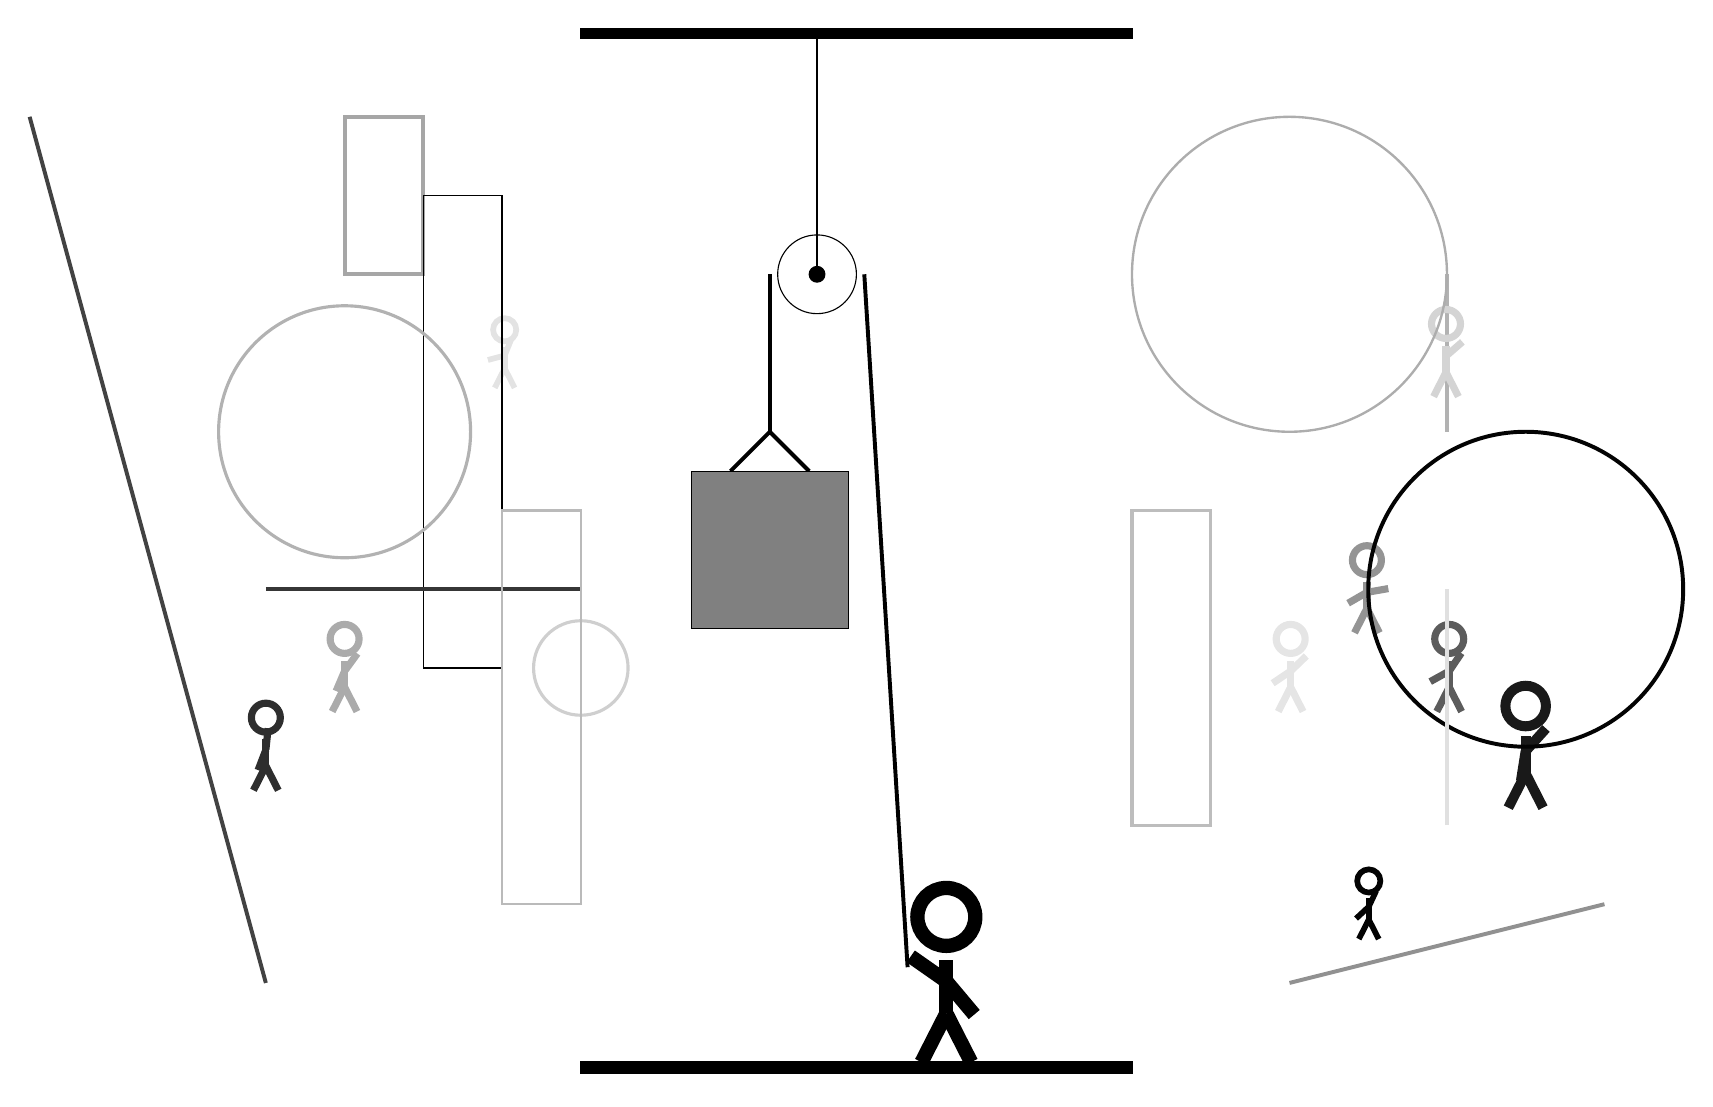
\begin{tikzpicture}
		%%%%% START %%%%%
		
		\draw[fill=black] (-2, 10) rectangle (5, 10.125);
		
		\draw[line width=0.3mm, color=black!80] (-3, -2) rectangle (-3, -2);
		
		\draw[line width=0.5mm, color=black!35] (-4, 7) rectangle (-5, 9);
		\node[line width=0.5mm, color=black!90] at (10, 1) {\Strichmaxerl[7][81][48]};
		\draw[line width=0.5mm, color=black!43](7, -2) -- (11, -1);
		
		\node[line width=0.4mm, color=black!11] at (-3, 6) {\Strichmaxerl[4][15][68]};
		\node[line width=0.7mm, color=black!82] at (-6, 1) {\Strichmaxerl[5][69][84]};
		\node[line width=0.6mm, color=black!33] at (-5, 2) {\Strichmaxerl[5][67][54]};
		
		\draw[line width=0.2mm, color=black!100] (-4, 8) rectangle (-3, 2);
		\draw [line width=0.3mm, color=black!91](7, 1) circle (0.0);
		\node[line width=0.7mm, color=black!99] at (8, -1) {\Strichmaxerl[4][43][65]};
		\draw[line width=0.5mm, color=black!30](9, 7) -- (9, 5);
		\draw[line width=0.5mm, color=black!79](-6, 3) -- (-2, 3);
		\node[line width=0.4mm, color=black!17] at (9, 6) {\Strichmaxerl[5][90][41]};
		\node[line width=0.5mm, color=black!10] at (7, 2) {\Strichmaxerl[5][34][44]};
		\draw[line width=0.5mm, color=black!74](-6, -2) -- (-9, 9);
		\node[line width=0.3mm, color=black!64] at (9, 2) {\Strichmaxerl[5][29][56]};
		\draw [line width=0.4mm, color=black!30](-5, 5) circle (1.6);
		\node[line width=0.4mm, color=black!42] at (8, 3) {\Strichmaxerl[5][30][10]};
		\draw [line width=0.5mm, color=black!99](10, 3) circle (2.0);
		\draw [line width=0.4mm, color=black!19](-2, 2) circle (0.6);
		\draw[line width=0.3mm, color=black!27] (-2, -1) rectangle (-3, 4);
		
		\draw[line width=0.5mm, color=black!12](9, 0) -- (9, 3);
		\draw[line width=0.4mm, color=black!26] (5, 0) rectangle (6, 4);
		\draw [line width=0.3mm, color=black!32](7, 7) circle (2.0);
		
		\draw (1, 7) circle (0.5);
		\draw[fill=black] (1, 7) circle (0.1);
		\draw (1, 10) -- (1, 7);
		
		\draw[line width=0.5mm] (-0.1, 4.5) -- (0.4, 5.0) -- (0.9, 4.5);
		\draw[fill=black!50] (-0.6, 4.5) rectangle (1.4, 2.5);
		
		\draw[line width=0.5mm] (0.4, 7) -- (0.4, 5.0);
		\centerarc[line width=0.5mm](1, 7)(0:180:0.6);
		\draw[line width=0.5mm](1.6, 7) -- (2.15, -1.8);
		
		\node at (2.6, -1.9) {\Strichmaxerl[10][-35][-50]};
		
		\draw[fill=black] (-2, -3) rectangle (5, -3.15);
		
		%%%%% END %%%%%
	\end{tikzpicture}
\end{document}